\documentclass{ximera}

 

\usepackage{epsfig}

\graphicspath{
  {./}
  {figures/}
}

\usepackage{morewrites}
\makeatletter
\newcommand\subfile[1]{%
\renewcommand{\input}[1]{}%
\begingroup\skip@preamble\otherinput{#1}\endgroup\par\vspace{\topsep}
\let\input\otherinput}
\makeatother

\newcommand{\includeexercises}{\directlua{dofile("/home/jim/linearAlgebra/laode/exercises.lua")}}

%\newcounter{ccounter}
%\setcounter{ccounter}{1}
%\newcommand{\Chapter}[1]{\setcounter{chapter}{\arabic{ccounter}}\chapter{#1}\addtocounter{ccounter}{1}}

%\newcommand{\section}[1]{\section{#1}\setcounter{thm}{0}\setcounter{equation}{0}}

%\renewcommand{\theequation}{\arabic{chapter}.\arabic{section}.\arabic{equation}}
%\renewcommand{\thefigure}{\arabic{chapter}.\arabic{figure}}
%\renewcommand{\thetable}{\arabic{chapter}.\arabic{table}}

%\newcommand{\Sec}[2]{\section{#1}\markright{\arabic{ccounter}.\arabic{section}.#2}\setcounter{equation}{0}\setcounter{thm}{0}\setcounter{figure}{0}}

\newcommand{\Sec}[2]{\section{#1}}

\setcounter{secnumdepth}{2}
%\setcounter{secnumdepth}{1} 

%\newcounter{THM}
%\renewcommand{\theTHM}{\arabic{chapter}.\arabic{section}}

\newcommand{\trademark}{{R\!\!\!\!\!\bigcirc}}
%\newtheorem{exercise}{}

\newcommand{\dfield}{{\sf dfield9}}
\newcommand{\pplane}{{\sf pplane9}}

\newcommand{\EXER}{\section*{Exercises}}%\vspace*{0.2in}\hrule\small\setcounter{exercise}{0}}
\newcommand{\CEXER}{}%\vspace{0.08in}\begin{center}Computer Exercises\end{center}}
\newcommand{\TEXER}{} %\vspace{0.08in}\begin{center}Hand Exercises\end{center}}
\newcommand{\AEXER}{} %\vspace{0.08in}\begin{center}Hand Exercises\end{center}}

% BADBAD: \newcommand{\Bbb}{\bf}

\newcommand{\R}{\mbox{$\Bbb{R}$}}
\newcommand{\C}{\mbox{$\Bbb{C}$}}
\newcommand{\Z}{\mbox{$\Bbb{Z}$}}
\newcommand{\N}{\mbox{$\Bbb{N}$}}
\newcommand{\D}{\mbox{{\bf D}}}
\usepackage{amssymb}
%\newcommand{\qed}{\hfill\mbox{\raggedright$\square$} \vspace{1ex}}
%\newcommand{\proof}{\noindent {\bf Proof:} \hspace{0.1in}}

\newcommand{\setmin}{\;\mbox{--}\;}
\newcommand{\Matlab}{{M\small{AT\-LAB}} }
\newcommand{\Matlabp}{{M\small{AT\-LAB}}}
\newcommand{\computer}{\Matlab Instructions}
\newcommand{\half}{\mbox{$\frac{1}{2}$}}
\newcommand{\compose}{\raisebox{.15ex}{\mbox{{\scriptsize$\circ$}}}}
\newcommand{\AND}{\quad\mbox{and}\quad}
\newcommand{\vect}[2]{\left(\begin{array}{c} #1_1 \\ \vdots \\
 #1_{#2}\end{array}\right)}
\newcommand{\mattwo}[4]{\left(\begin{array}{rr} #1 & #2\\ #3
&#4\end{array}\right)}
\newcommand{\mattwoc}[4]{\left(\begin{array}{cc} #1 & #2\\ #3
&#4\end{array}\right)}
\newcommand{\vectwo}[2]{\left(\begin{array}{r} #1 \\ #2\end{array}\right)}
\newcommand{\vectwoc}[2]{\left(\begin{array}{c} #1 \\ #2\end{array}\right)}

\newcommand{\ignore}[1]{}


\newcommand{\inv}{^{-1}}
\newcommand{\CC}{{\cal C}}
\newcommand{\CCone}{\CC^1}
\newcommand{\Span}{{\rm span}}
\newcommand{\rank}{{\rm rank}}
\newcommand{\trace}{{\rm tr}}
\newcommand{\RE}{{\rm Re}}
\newcommand{\IM}{{\rm Im}}
\newcommand{\nulls}{{\rm null\;space}}

\newcommand{\dps}{\displaystyle}
\newcommand{\arraystart}{\renewcommand{\arraystretch}{1.8}}
\newcommand{\arrayfinish}{\renewcommand{\arraystretch}{1.2}}
\newcommand{\Start}[1]{\vspace{0.08in}\noindent {\bf Section~\ref{#1}}}
\newcommand{\exer}[1]{\noindent {\bf \ref{#1}}}
\newcommand{\ans}{}
\newcommand{\matthree}[9]{\left(\begin{array}{rrr} #1 & #2 & #3 \\ #4 & #5 & #6
\\ #7 & #8 & #9\end{array}\right)}
\newcommand{\cvectwo}[2]{\left(\begin{array}{c} #1 \\ #2\end{array}\right)}
\newcommand{\cmatthree}[9]{\left(\begin{array}{ccc} #1 & #2 & #3 \\ #4 & #5 &
#6 \\ #7 & #8 & #9\end{array}\right)}
\newcommand{\vecthree}[3]{\left(\begin{array}{r} #1 \\ #2 \\
#3\end{array}\right)}
\newcommand{\cvecthree}[3]{\left(\begin{array}{c} #1 \\ #2 \\
#3\end{array}\right)}
\newcommand{\cmattwo}[4]{\left(\begin{array}{cc} #1 & #2\\ #3
&#4\end{array}\right)}

\newcommand{\Matrix}[1]{\ensuremath{\left(\begin{array}{rrrrrrrrrrrrrrrrrr} #1 \end{array}\right)}}

\newcommand{\Matrixc}[1]{\ensuremath{\left(\begin{array}{cccccccccccc} #1 \end{array}\right)}}



\renewcommand{\labelenumi}{\theenumi)}
\newenvironment{enumeratea}%
{\begingroup
 \renewcommand{\theenumi}{\alph{enumi}}
 \renewcommand{\labelenumi}{(\theenumi)}
 \begin{enumerate}}
 {\end{enumerate}\endgroup}



\newcounter{help}
\renewcommand{\thehelp}{\thesection.\arabic{equation}}

%\newenvironment{equation*}%
%{\renewcommand\endequation{\eqno (\theequation)* $$}%
%   \begin{equation}}%
%   {\end{equation}\renewcommand\endequation{\eqno \@eqnnum
%$$\global\@ignoretrue}}

%\input{psfig.tex}

\author{Martin Golubitsky and Michael Dellnitz}

%\newenvironment{matlabEquation}%
%{\renewcommand\endequation{\eqno (\theequation*) $$}%
%   \begin{equation}}%
%   {\end{equation}\renewcommand\endequation{\eqno \@eqnnum
% $$\global\@ignoretrue}}

\newcommand{\soln}{\textbf{Solution:} }
\newcommand{\exercap}[1]{\centerline{Figure~\ref{#1}}}
\newcommand{\exercaptwo}[1]{\centerline{Figure~\ref{#1}a\hspace{2.1in}
Figure~\ref{#1}b}}
\newcommand{\exercapthree}[1]{\centerline{Figure~\ref{#1}a\hspace{1.2in}
Figure~\ref{#1}b\hspace{1.2in}Figure~\ref{#1}c}}
\newcommand{\para}{\hspace{0.4in}}

\renewenvironment{solution}{\suppress}{\endsuppress}

\ifxake
\newenvironment{matlabEquation}{\begin{equation}}{\end{equation}}
\else
\newenvironment{matlabEquation}%
{\let\oldtheequation\theequation\renewcommand{\theequation}{\oldtheequation*}\begin{equation}}%
  {\end{equation}\let\theequation\oldtheequation}
\fi

\makeatother


\title{Exact Differential Equations}

\begin{document}
\begin{abstract}
\end{abstract}
\maketitle


\label{S:exact} 

We illustrate the idea behind exact equations with the following example:
\begin{equation}  \label{eq:exactex1}
\frac{dx}{dt} = \frac{x-1}{2x-t}.
\end{equation}
Since the right hand side of \eqref{eq:exactex1} is neither of the form 
$g(x)h(t)$ nor of the form $F\left(\frac{x}{t}\right)$, it cannot be 
solved either by separation of variables or by substitution.  However, 
it is possible to determine all solutions of \eqref{eq:exactex1}, as we now 
explain.

We may rewrite \eqref{eq:exactex1} as
\begin{equation} \label{eq:exactex1a}
(2x-t)\frac{dx}{dt} =(x-1). 
\end{equation}

Suppose that $x(t)$ is a solution to \eqref{eq:exactex1} and let 
$y(t)=x(t)^2 - x(t)t + t$.  Then differentiation shows that 
\[
\dot{y} = 2x\dot{x} -\dot{x}t-x + 1 = (2x-t)\dot{x} -(x-1) =0,
\]
with the last equality coming from \eqref{eq:exactex1a}.  Thus, if $x(t)$ is a 
solution, then the function $y(t)=x(t)^2 - x(t)t + t$ is constant.  It 
follows that for each solution $x(t)$ there is a real constant $c$ such that
\begin{equation} \label{eq:xc}
x(t)^2 - x(t)t + t = c.
\end{equation}
Since \eqref{eq:xc} is quadratic in $x$, the quadratic formula determines  
two solutions for each value of $c$, namely,
\begin{equation}  \label{E:twosolns}
x_\pm(t) = \frac{t\pm\sqrt{t^2-4t+4c}}{2}.
\end{equation}
When $c=1$, the radical in \eqref{E:twosolns} is a perfect square and the 
two solutions to \eqref{eq:exactex1} are:
\[
x_+(t) = t-1 \AND x_-(t) = 1,
\]
as can readily be checked. 

\subsubsection*{Solutions Lie on Level Contours}

To derive a geometric interpretation for the identity \eqref{eq:xc},
define the function $F:\R^2\rightarrow \R$ by
\[
F(t,x) = x^2 - xt + t.
\]
A {\em level set\/}\index{level set} or 
{\em contour\/}\index{contour} of $F$ is defined to be
the set of points in the $(t,x)$-plane for which
\[
F(t,x) = c,
\]
for some real constant $c$.  Thus, \eqref{eq:xc} can now be restated
as follows: solutions $x(t)$ of the differential equation \eqref{eq:exactex1} 
lie on the level sets of $F$, since $F(t,x(t))=c$.

\subsubsection*{Drawing Contours Using \Matlab}

We use the \Matlab command {\tt contour} to illustrate how this
information helps us to visualize all the solutions.  Type
\begin{verbatim}
[t,x] = meshgrid(-1.5:0.1:1.5,-1.5:0.1:1.5);
F = x.^2 - x.*t + t;
\end{verbatim}\index{\computer!meshgrid}
After these commands the data for the surface defined by the
function $F$ in the square $[-1.5,1.5]\times [-1.5,1.5]$ is
stored in the \Matlab variable {\tt F}.  The command {\tt
contour(F)}\index{\computer!contour} allows us to display 
the level sets\index{level set} of $F$.  To have
the correct scales on the axes, type
\begin{verbatim}
contour(t,x,F)
\end{verbatim}
Now the contour\index{contour} lines --- the level sets corresponding to
different levels $c$ --- are displayed.  Moreover, we want to know to which 
levels the curves in that picture belong.  Suppose that we are interested in 
the level sets corresponding to $c\in\{ -2,-1,0,1,2,3,4,5\}$.  Then we 
obtain this information by typing
\begin{verbatim}
cs = contour(t,x,F,[-2,-1,0,1,2,3,4,5]);
clabel(cs)
xlabel('t')
ylabel('x')
\end{verbatim}\index{\computer!contour}\index{\computer!clabel}
The command {\tt clabel} allows us to label the different
contour lines\index{contour!line} by their actual level.  The desired
information is displayed in Figure~\ref{Fig:contour1}.

\begin{figure}[htb]
           \centerline{%
           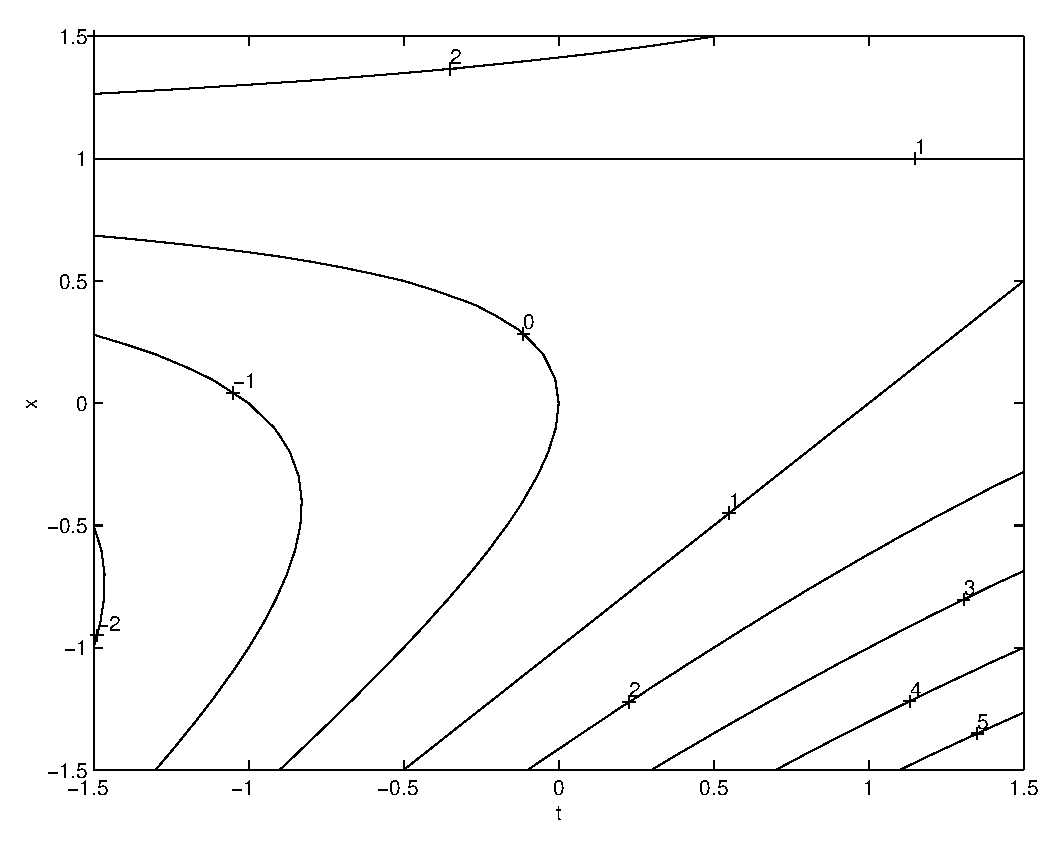
\psfig{file=../figures/contour1.eps,width=3.5in}}
           \caption{Contour lines of $F(t,x)=x^2-xt+t$ for
          $(t,x)\in[-1.5,1.5]\times[-1.5,1.5]$.}
           \label{Fig:contour1}
\end{figure}

Note that the straight line solutions $x(t)=1$ and $x(t)=t-1$ 
correspond to the level set for $c=1$, as expected.  We can also
see from Figure~\ref{Fig:contour1} that the contour lines for
the levels $c=0,-1,-2$ have a turning point, that is, they
cannot be parameterized entirely by $t$.  

Setting $c=0$ in \eqref{E:twosolns} we find the expressions
\[
x_+(t) = \frac{1}{2}\left(t+\sqrt{t(t-4)}\right) \AND
x_-(t) = \frac{1}{2}\left(t-\sqrt{t(t-4)}\right).
\]
These functions are not real-valued for $t\in (0,4)$.  In
particular, they cannot correspond to solutions of
\eqref{eq:exactex1} for these values of $t$.  This provides
an explanation for the existence of the turning point at
$(t,x)=(0,0)$ and why the solutions $x_+(t)$ and $x_-(t)$
``collide'' at this point.

Finally, we use {\dfield}\index{\computer!dfield8} to confirm our 
theoretical discussion.  We set the values in {\sf the display window}
as in Figure~\ref{Fig:contour1} and start the computation in 
\[
(t_0,x_0)=(-0.5,x_-(-0.5))=(-0.5,-1)
\]
using the {\sf Keyboard input}.  The result --- which is in good
agreement with the contour plot\index{contour!plot} --- is shown in
Figure~\ref{Fig:contour2}.  Observe that {\dfield} will not 
stop the computation of the forward orbit on its own and one has to
use the {\sf Stop} button to stop the numerical solution.  The reason is
that the program encounters numerical difficulties approaching the turning
point $(0,0)$, since the right hand side of the differential equation is
not defined at $(0,0)$.

\begin{figure}[htb]
  \centerline{%
  \psfig{file=../figures/contour2.eps,width=3.7in}}
  \caption{The solution of \protect\eqref{eq:exactex1} for the
  initial value $(t_0,x_0)=(-0.5,-1)$ computed by {\dfield}.}
  \label{Fig:contour2}
\end{figure}

\subsection*{The General Definition of Exact Differential Equations}

After this motivating example, we consider the general
situation.  Suppose that we have an ordinary differential
equation of the form
\begin{equation} \label{eq:exact}
\frac{dx}{dt} = \frac{G(t,x)}{H(t,x)},
\end{equation}
where $G$ and $H$ are real-valued continuous functions.  In 
\eqref{eq:exactex1}, $G(t,x)=x-1$ and $H(t,x) = 2x-t$.
The differential equation \eqref{eq:exact} is {\em exact\/} 
\index{differential equation!exact} if
there is a function $F(t,x)$ such that
\begin{equation}  \label{e:FGH}
\frac{\partial F}{\partial t} = -G \AND
\frac{\partial F}{\partial x} =  H.
\end{equation}
Indeed, the differential equation \eqref{eq:exactex1} is exact --- just set 
$F(t,x) = x^2 - xt + t$.

Supposing that the differential equation \eqref{eq:exact} is exact, proceed as 
in the example by rewriting \eqref{eq:exact} as 
\begin{equation} \label{eq:exacta}
H(t,x)\frac{dx}{dt} - G(t,x) = 0.
\end{equation}
Let $x(t)$ be a solution to \eqref{eq:exactex1} and use the chain rule, 
\eqref{e:FGH}, and \eqref{eq:exacta} to obtain
\[
\frac{d}{dt} F(t,x(t)) = \frac{\partial F}{\partial x}\frac{dx}{dt} + 
\frac{\partial F}{\partial t} = H\frac{dx}{dt}-G = 0.
\]
Hence, solutions of \eqref{eq:exact} must lie on a level set of $F$ defined 
by $F(t,x) = c$. We have proved:

\begin{theorem} \label{thm:exact}
Assume that the differential equation \eqref{eq:exact} is exact.  Then, for any 
solution $x(t)$ of \eqref{eq:exact} with $x(t_0)=x_0$, there is a constant $c$ 
such that for all $t$ close to $t_0$, $F(t,x(t)) = c$.
\end{theorem}\index{differential equation!exact}

\subsection*{On the Existence of $F$}

In order to solve exact differential equations,
\index{differential equation!exact} we must answer two 
questions: 
\begin{itemize}
\item When does a function $F$ exist that satisfies the 
conditions in \eqref{e:FGH}?
\item If the function $F$ exists, then how can we compute it?
\end{itemize}
The following proposition, based on the equality of mixed partial derivatives, 
gives a necessary condition for having a positive answer to the first question.

\begin{proposition} \label{prop:exact}
Let $G,H:\R^2\to\R$ be differentiable functions such that
$\partial G/\partial x$ and $\partial H/\partial t$ are
continuous.  Suppose that the corresponding differential
equation \eqref{eq:exact} is exact.  Then
\begin{equation} \label{eq:Gy=Hs}
-\frac{\partial G}{\partial x} (t,x) = \frac{\partial H}{\partial
t} (t,x).
\end{equation}
\end{proposition}

\begin{proof} Using \eqref{e:FGH} we compute
\[
\frac{\partial^2 F}{\partial x\partial t} = 
-\frac{\partial G}{\partial x} (t,x) \AND 
\frac{\partial^2 F}{\partial t\partial x} = 
\frac{\partial H}{\partial t} (t,x).
\]
Since $\partial G/\partial x$ and $\partial H/\partial t$ are
continuous, equality of mixed partial derivatives holds, and
\[
-\frac{\partial G}{\partial x} = 
\frac{\partial^2 F}{\partial x\partial t} =
\frac{\partial^2 F}{\partial t\partial x} =
\frac{\partial H}{\partial t},
\]
as desired. \end{proof}

\begin{remark} \label{rmk:exact}
{\rm It can be shown that criterion \eqref{eq:Gy=Hs} is also
sufficient for the exactness of the corresponding differential
equation, if this criterion is satisfied in a region in the
$(t,x)$-plane having no holes. The proof of this result can be
found in any text on multidimensional calculus.}
\end{remark}


\subsubsection*{Two Examples}

We use two examples to illustrate the test for exactness
\index{differential equation!exact!test for}
of the underlying differential equation given by \eqref{eq:Gy=Hs}.

\noindent (a) Consider \eqref{eq:exactex1}, that is, suppose $G(t,x)=x-1$ and 
$H(t,x)=2x-t$.  Then
\[
-\frac{\partial G}{\partial x} = -1 = 
\frac{\partial H}{\partial t},
\]
and according to Remark~\ref{rmk:exact} a function $F$ with the desired 
properties may be found.

\noindent (b) Suppose that $G(t,x) = 1$ and $H(t,x) = t$.  Then 
\[
-\frac{\partial G}{\partial x} (t,x) = 0\not= 1 = 
\frac{\partial H}{\partial t} (t,x),
\]
and by Proposition~\ref{prop:exact} a function $F$ satisfying \eqref{e:FGH} 
cannot exist.

\subsection*{On the Computation of $F$}
Next, consider the second question, namely, how can $F$ be
computed when it exists.  By \eqref{e:FGH} we have
\[
\frac{\partial F}{\partial t}(t,x) = -G(t,x).
\]
Therefore, there is a differentiable function $g:\R\to\R$ such
that
\begin{equation}  \label{eq:defGamma}
F(t,x) = -\Gamma(t,x) + g(x),
\end{equation}
where 
\[
\Gamma(t,x)=\int G(\tau,x) d\tau
\]
is an indefinite integral of $G$ with respect to the variable $t$.
Condition \eqref{e:FGH} also implies that
\[
H(t,x) = \frac{\partial F}{\partial x}(t,x) =
-\frac{\partial}{\partial x}\Gamma(t,x) + g'(x),
\]
that is
\begin{equation} \label{eq:defg}
g'(x) = \frac{\partial}{\partial x}\Gamma(t,x) + H(t,x).
\end{equation}
Equations \eqref{eq:defg} and \eqref{eq:defGamma} can now be used 
to compute the function $F$ as long as the corresponding
integrations can be performed.  

Equivalently, we can first integrate the condition $F_x=H$ to obtain
\begin{equation}  \label{eq:excond}
F(t,x) = \Omega(t,x) + h(t),
\end{equation}
where $\Omega(t,x)=\int H(t,x)dx$ is an indefinite integral of $H$ with
respect to $x$.  Then \eqref{e:FGH} leads to
\[
h'(t) = -\frac{\partial}{\partial t}\Omega(t,x) - G(t,x).
\]
In practice, we prefer one way to the other depending on which
integrations are easier to perform.

\subsubsection*{Two Examples}

\noindent (a) Reconsider \eqref{eq:exactex1}, that is, suppose $G(t,x)=x-1$ and 
$H(t,x)=2x-t$.  We can choose
\[
\Gamma(t,x)=\int G(\tau,y)d\tau = tx-t,
\]
and \eqref{eq:defg} becomes
\[
g'(x) = t + H(t,x) = 2x.
\]
We can then choose $g(x)=x^2$ and, by \eqref{eq:defGamma}, obtain
\[
F(t,x) = -\Gamma(t,x) + g(x) = -tx + t + x^2.
\]

\noindent (b) Next, consider the differential equation
\begin{equation}  \label{eq:exacex2}
\frac{dx}{dt} = \frac{2t(1-x^2)-x^6}{x(2t^2+3x+6tx^4)}.
\end{equation}
In our notation
\[
G(t,x) = 2t(1-x^2)-x^6 \AND H(t,x) = x(2t^2+3x+6tx^4).
\]
Therefore, 
\[
-\frac{\partial G}{\partial x} = 4tx + 6x^5 = 
\frac{\partial H}{\partial t}.
\]
Hence the equation is exact (see Proposition~\ref{prop:exact} and 
Remark~\ref{rmk:exact}).  

It is easier to compute $\Gamma(t,x)=\int G(\tau,x) d\tau$ than 
$\Omega(t,x)=\int H(s,x)dx$.  We choose 
\[
\Gamma(t,x) = t^2(1-x^2) - tx^6,
\]
and \eqref{eq:defg} becomes
\[
g'(x) = -(2t^2 x + 6tx^5) + x(2t^2+3x+6tx^4) = 3x^2.
\]
Now we use \eqref{eq:defGamma} to obtain
\[
F(t,x) = t^2(x^2-1) + tx^6 + x^3.
\]
Solutions of the differential equation \eqref{eq:exacex2} lie on
level sets of $F$.  In particular, the solution $x(t)$
determined by the initial condition $x(2)=1$ satisfies 
\[
F(t,x)=t^2(x^2-1) + tx^6 + x^3 = 3,
\]
since $F(2,1)=3$.  To see the qualitative behavior of the
solutions\index{contour!plot} we use the following sequence 
of \Matlab commands
\begin{verbatim}
[t,x] = meshgrid(1:0.02:3,0.5:0.01:1.5);
F  = t.^2.*(x.^2-1) + t.*x.^6 + x.^3;
cs = contour(t,x,F,[0,3,6,9,12]);
clabel(cs)
hold on
plot(2,1,'o')                  
xlabel('t')
ylabel('x')
\end{verbatim}\index{\computer!meshgrid}\index{\computer!contour}
\index{\computer!hold}\index{\computer!clabel}\index{\computer!plot}
The result is shown in Figure~\ref{Fig:contour3}.  

\begin{figure}[htb]
  \centerline{%
  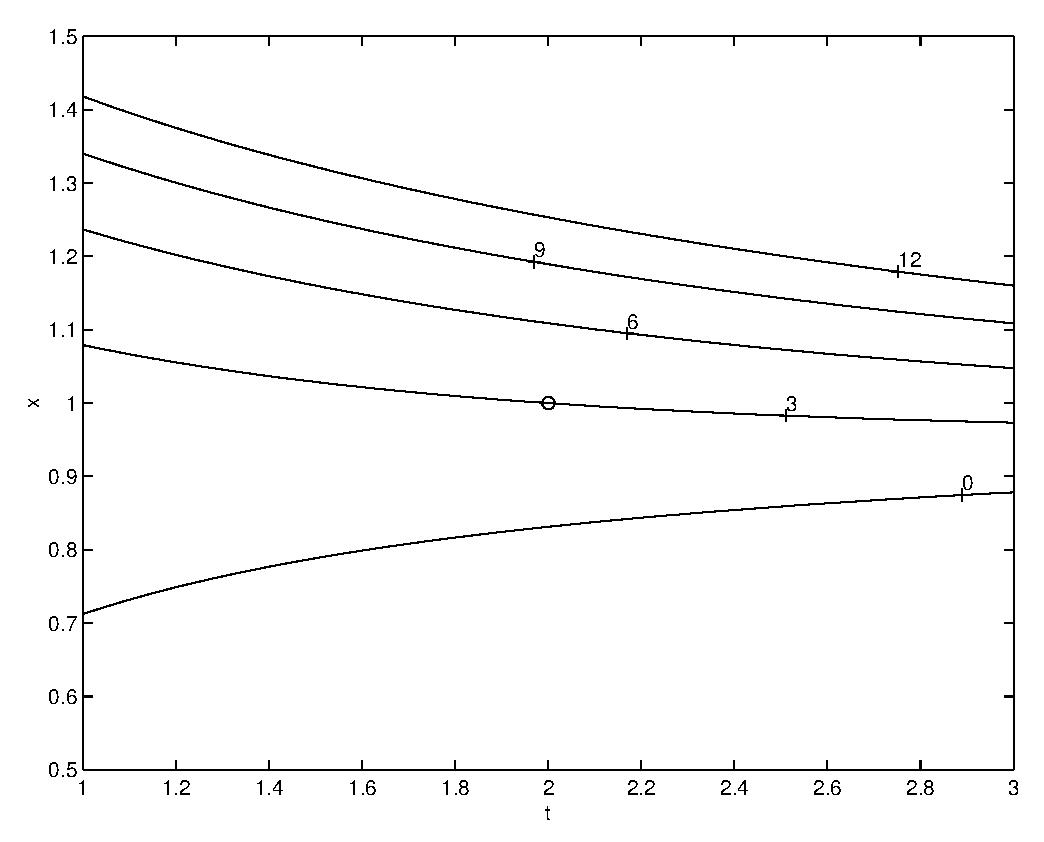
\psfig{file=../figures/contour3.eps,width=3.5in}}
  \caption{Solutions of the differential equation
\protect\eqref{eq:exacex2}
  corresponding to the levels $c=0,3,6,9,12$ in the rectangle
  $[1,3]\times [0.5,1.5]$.}
\label{Fig:contour3}
\end{figure}


\EXER

\TEXER

\noindent In Exercises~\ref{c14.6.2} -- \ref{c14.6.3} determine whether or 
not the given differential equations is exact.
\begin{exercise} \label{c14.6.2}
$\dps \frac{dx}{dt} = \frac{\cos x}{t\sin x}$.

\begin{solution}
\ans The differential equation is exact.

\soln We can write the differential equation as $\dps\frac{dx}{dt} =
\frac{G(t,x)}{H(t,x)}$, where $G(t,x) = \cos x$ and $H(t,x) = t\sin x$. 
Then we can compute
\[
-\frac{\partial G}{\partial x} = \sin x \AND
\frac{\partial H}{\partial t} = \sin x.
\]
By Proposition~\ref{prop:exact}, since the
two sides of \eqref{eq:Gy=Hs} are equal, the differential equation is exact.

\end{solution}
\end{exercise}
\begin{exercise} \label{c14.6.3}
$\dps \frac{dx}{dt} = \frac{\cos t}{x\sin t}$.

\begin{solution}
\ans The differential equation is not exact.

\soln We can write the differential equation as $\dps\frac{dx}{dt} =
\frac{G(t,x)}{H(t,x)}$, where $G(t,x) = \cos t$ and $H(t,x) = x\sin t$. 
Then we can compute
\[
-\frac{\partial G}{\partial x} = 0 \AND
\frac{\partial H}{\partial t} = x\cos t.
\]
By Proposition~\ref{prop:exact}, the differential equation is exact only
if the two sides of \eqref{eq:Gy=Hs} are equal.

\end{solution}
\end{exercise}

\begin{exercise} \label{c14.6.4}
Verify that the differential equation 
\[
\dps\frac{dx}{dt} = \dps \frac{2t-x}{t+1} 
\]
is exact and find a solution with initial value $x(0) = 3$.

\begin{solution}
\ans A solution to the initial value problem is
$x(t) = \dps\frac{3 + t^2}{1 + t}$.

\soln Write the differential equation as $\dps\frac{dx}{dt} =
\frac{G(t,x)}{H(t,x)}$, where $G(t,x) = 2t - x$ and $H(t,x) = t + 1$.  Then,
since
\[
-\frac{\partial G}{\partial x} = 1 = \frac{\partial H}{\partial t},
\]
the differential equation is exact, by
Proposition~\ref{prop:exact}.  Next, we must find a function $F(t,x)$
satisfying \eqref{eq:excond}.  By integration, obtain
\[
\Omega(t,x) = \int H(t,x)dy = \int (t + 1)dx = (t + 1)x.
\]
Then, find the function $h(t)$ such that
\[
h'(t) = -\frac{\partial}{\partial t}\Omega(t,x) - G(t,x)
= -2t.
\]
In this case, $h(t) = -t^2$.  Finally, compute
\[
F(t,x) = \Omega(t,x) + h(t) = tx + x - t^2,
\]
the function satisfying \eqref{eq:excond}.  Now, substitute the initial
condition $(t,x) = (0,3)$ into $F(t,x)$, obtaining $F(0,3) = 3$.  Thus,
$x(t)$ satisfies
\[
tx + x - t^2 = 3.
\]
Solve for $x$ to find the solution to the initial value problem.

\end{solution}
\end{exercise}

\begin{exercise} \label{c14.6.6}
Verify that the differential equation 
\[
\frac{dx}{dt} = \frac{x}{x-t}
\]
is exact and find a solution with initial value $x(2)=3$.   Compare your 
answer with Exercise~\ref{exer:at} in Section~\ref{S:3.2}.

\begin{solution}
\ans A solution to the initial value problem is
\[
x(t) = t + \sqrt{t^2-3}.
\]

\soln Write the differential equation as $\dps\frac{dx}{dt} =
\frac{G(t,x)}{H(t,x)}$, where $G(t,x) = x$ and $H(t,x) = x - t$.  Then,
since
\[
-\frac{\partial G}{\partial x} = -1 = \frac{\partial H}{\partial t},
\]
the differential equation is exact by Proposition~\ref{prop:exact}.  Next,
we must find a function $F(t,x)$ satisfying \eqref{eq:excond}.  By integration,
obtain
\[
\Omega(t,x) = \int H(t,x)dy = \int (x - t)dx = \frac{1}{2}x^2 -tx.
\]
Then, find the function $h(t)$ such that
\[
h'(t) = -\frac{\partial}{\partial t}\Omega(t,x) - G(t,x)
= x - x = 0 .
\]
In this case, we can choose $h(t) = 0$.  Finally, compute
\[
F(t,x) = \Omega(t,x) + h(t) =  \frac{1}{2}x^2 -tx,
\]
the function satisfying \eqref{eq:excond}.  Now, substitute the initial
condition $(t,x) = (2,3)$ into $F(t,x)$, obtaining $F(2,3) = -\frac{3}{2}$.  Thus,
$x(t)$ satisfies
\[
 \frac{1}{2}x^2 -tx = -\frac{3}{2}.
\]
Solve for $x$ to find the solution to the initial value problem.  The
solution is exactly the one given in Exercise~\ref{exer:at} from
Section~\ref{S:3.2}.


\end{solution}
\end{exercise} 

\begin{exercise}  \label{ex:if}
Show that the differential equation
\begin{equation} \label{Ex:nexact}
\frac{dx}{dt} = -\frac{1+3tx}{t^2}
\end{equation}
is not exact.  Now multiply both the numerator and denominator of the 
right side of \eqref{Ex:nexact} by $t$ and show that this `new' differential
equation 
\[
\frac{dx}{dt} = -\frac{t+3t^2x}{t^3}
\]
is exact. Now find all solutions to \eqref{Ex:nexact}.

\begin{solution}
\ans The general solution is 
\[ x = \frac{C}{t^3} - \frac{1}{2t} \] 
for some constant $C$.

\soln We can write the differential equation as $\dps\frac{dx}{dt} =
\frac{G(t,x)}{H(t,x)}$, where $G(t,x) = -1-3tx$ and $H(t,x) = t^2$. 
Then we compute
\[
-\frac{\partial G}{\partial x} = 3t \AND
\frac{\partial H}{\partial t} = 2t.
\]
By Proposition~\ref{prop:exact}, the
differential equation is exact only if the two sides of \eqref{eq:Gy=Hs} are
equal.
On multiplying numerator and denominator by $t$ we obtain
where $G(t,x) = -t-3t^2x$ and $H(t,x) = t^3$. 
Then we compute
\[
-\frac{\partial G}{\partial x} = 3t^2 \AND
\frac{\partial H}{\partial t} = 3t^2.
\]
So the new form of the differential equation is exact.

Next, we must find a function $F(t,x)$ satisfying \eqref{eq:excond}.
By integration, obtain
\[
\Omega(t,x) = \int H(t,x)dx = \int t^3dx = t^3x.
\]
Then, find the function $h(t)$ such that
\[
h'(t) = -\frac{\partial}{\partial t}\Omega(t,x) - G(t,x)
= t.
\]
In this case, we can choose 
\[
h(t) =  \frac{1}{2}t^2.  
\]
Finally, compute
\[
F(t,x) = \Omega(t,x) + h(t) = t^3x + \frac{1}{2}t^2,
\]
the function satisfying \eqref{eq:excond}.  The general solution is found by 
solving $F=C$ for $x$; that is, solving
\[
\frac{1}{2}t^2 + t^3x = C.
\]

\end{solution}
\end{exercise}

\begin{exercise}  \label{ex:if2}
Show that the differential equation
\begin{equation} \label{Ex:nexact2}
\frac{dx}{dt} = -\frac{3x}{2t}
\end{equation}
is not exact.  Now multiply both the numerator and denominator of the 
right side of \eqref{Ex:nexact2} by $t^2x$ and show that this `new' differential
equation 
\[
\frac{dx}{dt} = -\frac{3t^2x^2}{2t^3x}
\]
is exact.  Now find all solutions to \eqref{Ex:nexact2}.

\begin{solution}
\ans The general solution is $x = \dps\pm\sqrt{\frac{C}{3t^3}}$ 
for some constant $C$.

\soln We can write the differential equation as $\dps\frac{dx}{dt} =
\frac{G(t,x)}{H(t,x)}$, where $G(t,x) = -3x$ and $H(t,x) = 2t$. 
Then we compute
\[
-\frac{\partial G}{\partial x} = 3 \AND
\frac{\partial H}{\partial t} = 2.
\]
By Proposition~\ref{prop:exact}, the differential equation is exact only
if the two sides of \eqref{eq:Gy=Hs} are equal.
On multiplying numerator and denominator by $t^2x$ we obtain
where $G(t,x) = -3t^2x^2$ and $H(t,x) = 2t^3x$. 
Then we compute
\[
-\frac{\partial G}{\partial x} = 6t^2x \AND
\frac{\partial H}{\partial t} = 6t^2x.
\]
So the new form of the differential equation is exact.

Next, we must find a function $F(t,x)$ satisfying \eqref{eq:excond}.  By
integration, obtain
\[
\Omega(t,x) = \int H(t,x)dx = \int 2t^3xdx = t^3x^2.
\]
Then, find the function $h(t)$ such that
\[
h'(t) = -\frac{\partial}{\partial t}\Omega(t,x) - G(t,x)
= 6t^2x^2.
\]
In this case, we can choose 
\[
h(t) =  2t^3x^2.  
\]
Finally, compute
\[
F(t,x) = \Omega(t,x) + h(t) = 3t^3x^2,
\]
the function satisfying \eqref{eq:excond}.  The general solution is found by 
solving $F=C$ for $x$; that is, solving
\[
3t^3x^2 = C.
\]

\end{solution}
\end{exercise}

\begin{exercise} \label{c14.6.7}
Let $G,H:\R^2\to\R$ be continuous functions and suppose that the differential 
equation 
\begin{equation}  \label{eq:if1}
\frac{dx}{dt} = \frac{G(t,x)}{H(t,x)}
\end{equation}
is {\bf not} exact.   An {\em integrating factor\/} for \eqref{eq:if1} is 
a function $\rho:\R^2\rightarrow\R$ such that the differential equation
\[
\frac{dx}{dt} = \frac{\rho(t,x) G(t,x)}{\rho(t,x)H(t,x)}
\]
is exact.  Suppose that there exists an integrating factor $\rho(t)$ for 
\eqref{eq:if1} that is a function of $t$ alone.  Show that $\rho$ satisfies
\[
\frac{d\rho}{dt} = -\frac{\rho}{H}
\left( \frac{\partial G}{\partial x}+\frac{\partial H}{\partial t}\right).
\]

\begin{solution}

Suppose that $\rho(t)$ is an integrating factor for the differential equation
\[
\frac{dx}{dt}(t) = \frac{G(x,t)}{H(x,t)}=\frac{\rho(t)G(x,t)}{\rho(t)H(x,t)}.
\]
That is,
\[
-\frac{d}{dx}(\rho(t)G(x,t)) = \frac{d}{dt}(\rho(t)H(x,t)).
\]
Differentiation yields
\[
-\rho(t)G_x(x,t) = \rho_t(t)H(x,t) + \rho(t)H_t(x,t).
\]
Therefore,
\begin{equation} \label{EX:if}
\rho_t = -\rho\frac{G_x+H_t}{H},
\end{equation}
as claimed.

\end{solution}
\end{exercise}

\begin{exercise} \label{c14.6.7A}
Use the result of Exercise~\ref{c14.6.7} to find an integrating factor for 
the differential equation
\[
\frac{dx}{dt} = -\frac{8x+5t}{4t},
\]
and then determine all solutions of this differential equation.

\begin{solution}
\ans $x(t) = \dps\frac{C}{4t^2} - \frac{5}{12}t$.

\soln  For the given differential equation $G(x,t)=-8x-5t$ and $H(x,t)=4t$. 
Since $-G_x=8$ and $H_t=4$, it follows that the differential equation is not
exact.  We solve (\ref{EX:if}) for an integrating factor $\rho(t)$.  That is,
we solve
\[
\rho_t = -\rho\frac{-8+4}{4t} = \frac{1}{t}\rho.
\]
We can use separation of variable to solve this equation.  That is,
\[
\frac{\rho_t}{\rho} =  \frac{1}{t}.
\]
On integration we find that $\rho=t$ is a solution.

To verify that $\rho(t)=t$ is an integrating factor, let $G(x,t)=-8xt-5t^2$
and $H(x,t)=4t^2$.  Then 
\[
-G_x = 8t \AND H_t = 8t,
\]
so that this equation is exact.

Next, we must find a function $F(t,x)$ satisfying \eqref{eq:excond}.  By
integration, obtain
\[
\Omega(t,x) = \int H(t,x)dx = \int 4t^2dx = 4t^2x.
\]
Then, find the function $h(t)$ such that
\[
h'(t) = -\frac{\partial}{\partial t}\Omega(t,x) - G(t,x) = 5t^2.
\]
In this case, we can choose 
\[
h(t) =  \frac{5}{3}t^3.  
\]
Finally, compute
\[
F(t,x) = \Omega(t,x) + h(t) = 4t^2x + \frac{5}{3}t^3,
\]
the function satisfying \eqref{eq:excond}.  The general solution is found by 
solving $F=C$ for $x$; that is, solving
\[
4t^2x + \frac{5}{3}t^3 = C.
\]

\end{solution}
\end{exercise}

\CEXER


\begin{exercise} \label{c14.6.8}
Consider the differential equation
\[
\frac{dx}{dt} = -\frac{2tx+\cos x}{t(t-\sin x)}.
\]
Show that this differential equation is 
exact.  Then use the command {\tt contour}\index{\computer!contour} in \Matlab 
to find solutions.  For the display, 
use the rectangle $[-2,2]\times [-2,2]$ in the $(t,x)$-plane and show contour
lines for the different levels $c=-4,-3,-2,-1,0,1,2,3,4$.  Mark the solution
which satisfies the initial condition $x(1)=0$ by a circle.
{\bf Hint:} Use the same procedure that was used to create 
Figure~\ref{Fig:contour3}.

\begin{solution}
The equation is exact, since it is of the form
$\dps\frac{dx}{dt} = \frac{G(t,x)}{H(t,x)}$ with
$-G=\dps\frac{\partial F}{\partial t}$ and
$H=\dps\frac{\partial F}{\partial x}$ for $F(t,x) = t^2 x + t\cos(x)$.
Now type the commands
\begin{verbatim}
[t,x] = meshgrid(-2:0.05:2,-2:0.05:2);
F = t.^2.*x + t.*cos(x);
cs = contour(t,x,F,[-4,-3,-2,-1,0,1,2,3,4]);
clabel(cs)
hold on
plot(1,0,'o')
xlabel('t')
ylabel('x')
\end{verbatim}
The result is given in Figure~\ref{c14.6.8}.
\begin{figure}[htb]
     \centerline{%
     \psfig{file=exfigure/fig17-6-9.eps,width=3.0in}}
        \exercap{c14.6.8}
\end{figure} 




\end{solution}
\end{exercise}


\end{document}
